\documentclass[pdflatex,11pt]{aghdpl}
% \documentclass{aghdpl}               % przy kompilacji programem latex
% \documentclass[pdflatex,en]{aghdpl}  % praca w j�zyku angielskim
\usepackage[polish]{babel}

\usepackage{polski}

\usepackage[cp1250]{inputenc}


% dodatkowe pakiety
\usepackage{enumerate}
\usepackage{listings}
\usepackage{mathtools}
\usepackage{bigstrut}
\usepackage{rotating}
\usepackage{multirow}
\usepackage{tocloft}
\usepackage{graphicx}
\usepackage{caption}
\usepackage{subcaption}
\usepackage{float}
\lstloadlanguages{TeX}

%\numberwithin{equation}{section}

%---------------------------------------------------------------------------

\author{Jakub Gola, Zbigniew Tekiela}
\shortauthor{J. Gola, Z. Tekiela}

\titlePL{Metody inicjalizacji modelu t�a}
\titleEN{Background model initialization methods}

\shorttitlePL{Metody inicjalizacji modelu t�a} % skr�cona wersja tytu�u je�li jest bardzo d�ugi
\shorttitleEN{Background model initialization methods}

\thesistypePL{Praca in�ynierska}
\thesistypeEN{Bachelor of Science Thesis}

\supervisorPL{dr hab. in�. Marek Gorgo�}
\supervisorEN{Marek Gorgo� Ph.D }

\date{2012}

\departmentPL{Katedra Automatyki}
\departmentEN{Department of Automatics}

\facultyPL{Wydzia� Elektrotechniki, Automatyki, Informatyki i In�ynierii Biomedycznej}
\facultyEN{Faculty of Electrical Engineering, Automatics, Computer Science and Biomedical Engineering}

\acknowledgements{Serdecznie dzi�kuj� \dots tu ci�g dalszych podzi�kowa� np. dla promotora, �ony, s�siada itp.}



\setlength{\cftsecnumwidth}{10mm}
\setcounter{tocdepth}{3}
\setcounter{secnumdepth}{4}
%---------------------------------------------------------------------------

\begin{document}

\titlepages

\tableofcontents
\clearpage

\chapter{Wst�p}
\label{wstep}

W dzisiejszych czasach systemy wizyjne znajduj� coraz wi�cej zastosowa� w~�yciu codziennym. Wraz ze wzrostem mocy obliczeniowej wsp�czesnych komputer�w oraz spadkiem cen kamer i~sprz�tu wizyjnego mo�na zaobserwowa� dynamiczny rozw�j tej dziedziny informatyki. S� one u�ywane mi�dzy innymi w~systemach inteligentnego, obszarowego sterowania ruchem, monitoringu przestrzeni miejskiej oraz w~bardziej zaawansowanych rozwi�zaniach CCTV, jak na przyk�ad systemach detekcji potencjalnych zagro�e� na lotniskach lub w~miejscach publicznych. We wszystkich wy�ej wymienionych zastosowaniach kluczow� kwesti� jest oddzielenie pierwszego planu od t�a. Odseparowanie dynamicznych element�w obrazu od statycznej scenerii jest podstaw� dzia�ania znacznej cz�ci algorytm�w �ledz�cych.

W tym miejscu nale�y zwr�ci� uwag� na r�nic� pomi�dzy inicjalizacj�, a generacj� t�a. Inicjalizacja modelu t�a jest to proces jednorazowy, w kt�rym na podstawie pewnej liczby ramek i odpowiednich algorytm�w zostaje uzyskany model t�a. Generacj� t�a natomiast nazywany jest ci�g�y proces aktualizacji wst�pnie zainicjalizowanego modelu  t�a. W algorytmach generacji t�a po��dana jest mo�liwo�� wykonywania ich w czasie rzeczywistym, natomiast przy inicjalizacji t�a czas dzia�ania algorytmu jest mniej istotny. We wszystkich algorytmach generacji t�a wyst�puje inicjalizacja, jednak�e w wielu z nich jest ona bardzo ograniczona  i~polega na uznaniu pierwszej ramki jako pierwszego modelu t�a.

Pomimo ci�g�ego rozwoju algorytm�w stosowanych do inicjalizacji modelu t�a nadal istniej� sytuacje, w~kt�rych algorytmy te nie s� w~stanie wygenerowa� poprawnych rezultat�w. Najwi�ksze problemy sprawiaj� zmienne warunki o�wietlenia oraz drobne ruchy obiekt�w t�a (np. li�cie na wietrze). Kolejnym niepo��danym zjawiskiem jest wtapianie si� obiekt�w z~pierwszego planu w~t�o, gdy pozostaj� one przez d�ugi czas nieruchome. 
Nieustannie trwaj� prace nad stworzeniem algorytm�w eliminuj�cych lub minimalizuj�cych skutki wy�ej wymienionych zjawisk. Pr�by te zosta�y opisane mi�dzy innymi w~\cite{Baltieri2010} oraz \cite{Reddy2009}.
Metody te zaliczaj� si� do klasy metod przestrzennych (blokowych), a~ich zaimplementowanie i~por�wnanie b�dzie stanowi� jeden z~cel�w niniejszej pracy. Nast�pnie zostan� one skonfrontowane z~metodami operuj�cymi na poziomie pikseli - opisanymi w~pracach \cite{7}.
\newpage
\section{Struktura pracy i stworzone programy}
Niniejsza praca sk�ada si� z nast�puj�cych rozdzia��w (w nawiasach podano osob� odpowiedzialn� za dany rozdzia�):
\begin{enumerate}
\item Wst�p - wprowadzenie do zagadnienia, zastosowania metod inicjalizacji modelu t�a (Jakub Gola, Zbigniew Tekiela),
\item Metody operuj�ce na poziomie pikseli - opis metod MOG, �rednia z~bufora ramek, mediana z~bufora ramek, aproksymacja �redniej przy u�yciu parametru alfa (Zbigniew Tekiela),
\item Metody blokowe (przestrzenne) - opis metod operuj�cych na grupach pikseli, wykorzystuj�cych transformat� DCT i rekursywn� transformat� Hadamarda (Jakub Gola),
\item Metodologia bada� - opis u�ytych sekwencji wideo oraz metryk do oceny skuteczno�ci metod (Jakub Gola, Zbigniew Tekiela),
\item Badania - opis rezultat�w uzyskanych przez poszczeg�lne metody (Jakub Gola - metody przestrzenne, Zbigniew Tekiela - metody operuj�ce na pikselach),
\item Por�wnanie metod - opis por�wnawczy metod MOG, mediana z bufora i metod przestrzennych, por�wnanie warto�ci metryk (Jakub Gola, Zbigniew Tekiela),
\item Wnioski - om�wienie rezultat�w uzyskanych przez poszczeg�lne metody, propozycje ulepsze� algorytm�w (Jakub Gola, Zbigniew Tekiela),
\item S�ownik u�ytych poj�� - obja�nienia termin�w u�ywanych w niniejszej pracy (Jakub Gola),
\item Dodatek A - spis zawarto�ci p�yty CD (Zbigniew Tekiela),
\item Dodatek B - opis najwa�niejszych klas i metod u�ytych program�w (Jakub Gola - program robust.exe, Zbigniew Tekiela - program simple\_pixel\_methods).
\end{enumerate}

W celu por�wnania metod inicjalizacji t�a utworzono nastepuj�ce programy (w nawiasie podano osob� odpowiedzialn�):
\begin{enumerate}
\item robust.exe - program obliczaj�cy model t�a metodami przestrzennymi (Jakub Gola) oraz metod� MOG (Zbigniew Tekiela),
\item simple\_pixel\_methods.exe - program obliczaj�cy model t�a metodami: �redniej z bufora ramek (Jakub Gola), aproksymacji �redniej przy u�yciu parametru alfa, mediany z bufora ramek (Zbigniew Tekiela).
\end{enumerate}
\chapter{Metody operuj�ce na poziomie pikseli}
\label{cha:Metody operuj�ce na poziomie pikseli}
\section{Mixture of Gaussians (MOG)}
\subsection{Wprowadzenie}
T�o sceny zawiera wiele dynamicznych obiekt�w jak poruszane na wietrze ga��zie i~li�cie drzew czy krzew�w. Zmiany w~obrazie nimi wywo�ane powoduj�, �e warto�� intensywno�ci danego piksela oraz jego kolor w~czasie mog� si� bardzo r�ni� od siebie. Z~tego powodu wykorzystanie pojedynczego przybli�enia rozk�adu prawdopodobie�stwa przy u�yciu krzywej Gaussa daje z�e rezultaty. Zamiast tego w~opisywanej metodzie u�yto podej�cia bazuj�cego na wykorzystaniu kilku rozk�ad�w Gaussa o~r�nych parametrach w~celu zamodelowania takich zmian \cite{7}.

Standardowe adaptacyjne modele t�a polegaj� na tworzeniu aproksymacji t�a, kt�re jest podobne do obecnej statycznej sceny za wyj�tkiem miejsc, w~kt�rych odby� si� ruch. Podej�cie takie jest efektywne w~sytuacjach, gdy obiekty poruszaj� si� stale, a~t�o jest widoczne znaczn� cz�� czasu, jednak�e nie sprawdza si� ono dla scen zawieraj�cych du�o poruszaj�cych si� obiekt�w, a~w szczeg�lno�ci, gdy obiekty te poruszaj� si� powoli. Nie potrafi tak�e poradzi� sobie z~t�ami posiadaj�cymi rozk�ad dwumodalny, powoli odtwarza t�o je�li zostanie ono odkryte i~ma jeden ustalony pr�g dla ca�ej sceny. 

W metodzie MOG zamiast modelowa� warto�ci wszystkich pikseli jako wy��cznie jeden typ rozk�adu, modelowane s� one mieszank� rozk�ad�w Gaussa. Bazuj�c na wadze i~wariancji ka�dego u�ytego do mieszanki rozk�adu Gaussa okre�lane jest, kt�re z~nich mog� odnosi� si� do kolor�w t�a. Warto�ci pikseli, kt�re nie mieszcz� si� w~�adnym rozk�adzie t�a uznawane s� za piksele nale��ce do pierwszego planu. Taki stan pikseli utrzymuje si� do czasu kiedy zaczn� wystarczaj�co dobrze pasowa� do kt�rego� z~rozk�ad�w t�a. 

Opisywana metoda dostosowuje si� aby radzi� sobie ze zmianami o�wietlenia, powtarzalnymi ruchami element�w t�a, powolnie poruszaj�cymi si� elementami pierwszego planu oraz wprowadzaniu lub usuwaniu element�w ze sceny. Powolnie poruszaj�ce si� elementy potrzebuj� wi�cej czasu aby wpasowa� si� w~t�o, poniewa� rozk�ad do kt�rego pasuj� ma wi�ksz� wariancj� ni� t�o. Powtarzaj�ce si� zmiany r�wnie� s� uwzgl�dniane, a~model rozk�adu t�a jest utrzymywany nawet je�li jest chwilowo zamieniony przez inny rozk�ad, co prowadzi do szybszego odtworzenia t�a w~przypadku usuni�cia obiekt�w ze sceny.
Metoda ta wykorzystuje dwa podstawowe parametry: 
\begin{lstlisting}
a - sta�a uczenia
T - porcja danych jaka powinna by� uwzgl�dniona w~tle
\end{lstlisting}

Zak�adaj�c, �e ka�dy piksel obrazu b�dzie pochodzi� z~jednej p�aszczyzny przy zmiennym �wietleniu, to do wydzielenia t�a z~takiego obrazu wystarczy u�ycie pojedynczej adaptacyjnej aproksymacji rozk�adem Gaussa dla ka�dego piksela. Jednak�e w~rzeczywistych warunkach na obrazie wyst�puje wiele powierzchni oraz zmienne o�wietlenie, co sprawia, �e potrzebne staje si� u�ycie kilku adaptacyjnych rozk�ad�w Gaussa. W~opisywanej metodzie u�yta jest mieszanka kilku takich rozk�ad�w o~r�nych parametrach. Za ka�dym razem, gdy parametry rozk�adu s� aktualizowane, nast�puje proces oceny dost�pnych rozk�ad�w w~celu okre�lenia tego najbardziej prawdopodobnego. 

\subsection{Opis metody}
\subsubsection{Model mieszanki}

Niech kolejne warto�ci danego piksela w~czasie nazywaj� si� histori� piksela. Zatem historia piksela jest to seria warto�ci danego piksela, gdzie dla obraz�w w~skali szaro�ci s� to warto�ci skalarne, a~dla obraz�w kolorowych s� to wektory. O~danym pikselu $\{x_0,y_0\}$ w~danej chwili czasu t, mo�na powiedzie�, �e znana jest jego historia
\begin{equation}
\{X_1,\dots,X_t\}=\{I(x_0,y_0,i):1\le i \le t\}
\end{equation}
gdzie $I$ jest sekwencj� ramek.

Niedawna historia dla ka�dego piksela modelowana jest mieszank� K~rozk�ad�w Gaussa. Prawdopodobie�stwo zaobserwowania obecnego piksela okre�la si� wzorem

\begin{equation}
P(X_t)=\sum_{i=1}^{K} \omega_{i,t} * \eta(X_t, \mu_{i,t} , \Sigma_{i,t})
\end{equation}

\noindent gdzie K~jest liczb� rozk�ad�w,  $\omega_{i,t}$ jest oszacowan� wag� $i$-tego rozk�adu w~mieszance w~chwili $t$, $\mu_{i,t}$ jest �redni� warto�ci�  $i$-tego rozk�adu w~mieszance w~chwili $t$, $\Sigma_{i,t}$ jest macierz� kowariancji w~chwili $t$,$\eta$ jest funkcj� g�sto�ci prawdopodobie�stwa Gaussa:

\begin{equation}
\eta(X_t,\mu,\Sigma)=\frac{1}{(2\pi)^\frac{n}{2} |\Sigma|^\frac{1}{2}}e^{-\frac{1}{2}(X_t-\mu_t)^T \Sigma^{-1} (W_t -\mu_t)}
\end{equation}

\noindent gdzie K~okre�lane jest przez dost�pn� pami�� oraz moc obliczeniow� jednostki na kt�rej wykonywany jest algorytm. Najcz�ciej spotykana warto�� mie�ci si� w~zakresie od 3~do 5. W~celu zmniejszenia ilo�ci oblicze� przyjmuje si�, �e macierz kowariancji ma posta�:

\begin{equation}
\Sigma_{k,t}=\sigma^2_kI
\end{equation}

Takie rozwi�zanie zak�ada, �e warto�ci dla poszczeg�lnych sk�adowych barwnych ka�dego piksela maj� tak� sam� wariancj�. Za�o�enie to obci��one jest pewnymi b��dami, lecz pozwala unikn�� wykonywania operacji odwracania macierzy, co jest zadaniem bardzo kosztownym, za cen� mniejszej precyzji. 

Zatem rozk�ad ostatnio obserwowanych warto�ci dla ka�dego piksela w~obrazie opisany jest mieszank� rozk�ad�w Gaussa. Nowa warto�� piksela b�dzie na og� reprezentowana przez jeden z~g��wnych sk�adnik�w mieszanki. 

Do obliczenia warto�ci nowego piksela u�yta zosta�a metoda on-line K-means approximation. Ka�da warto�� piksela jest sprawdzana pod k�tem dopasowania do jednego z~K rozk�ad�w. Warunkiem przynale�no�ci jest warto�� w~zakresie do 2,5 odchylenia standardowego z~danego rozk�adu. Zmiana opisanego wcze�niej progu ma niewielki wp�yw na wydajno�� algorytmu. Opisany spos�b wyboru odpowiednich pikseli jest bardzo u�yteczny dla obszar�w z~r�nym o�wietleniem, poniewa� obiekty znajduj�ce si� w~zacienionych obszarach maj� mniejszy szum ni� obiekty znajduj�ce si� w~ja�niejszych regionach.

W przypadku, gdy �aden rozk�ad nie zosta� dopasowany do danego piksela, to rozk�ad z~najmniejsz� wag� jest zast�powany nowym z~warto�ci� piksela jako now� warto�ci� oczekiwan�, du�� wariancj� i~nisk� wag�.

Wcze�niejsze wagi K~rozk�ad�w w~czasie t~s� aktualizowane wg wzoru: 

\begin{equation}
\omega_{k,t}=(1-\alpha)\omega_{k,t-1}+\alpha(M_{k,t})
\end{equation}
gdzie: $\alpha$ to tempo uczenia, a~$M_{k,t}$ jest 1~dla dopasowanego rozk�adu i~0 dla pozosta�ych rozk�ad�w. Po dokonaniu aproksymacji wagi s� normalizowane. $\frac{1}{\alpha}$ oznacza sta�� czasow� okre�laj�c� pr�dko�� z~jak� parametry rozk�ad�w si� zmieniaj�.

Dla rozk�ad�w niedopasowanych do danego piksela warto�ci $\mu$ i~$\sigma$ pozostaj� niezmienione. Dla rozk�ad�w, kt�re zosta�y dopasowane warto�ci $\mu$ i~$\sigma$ obliczane s� nast�puj�co:

\begin{equation}
\mu_t=(1-\rho)\mu_{t-1}+\rho X_t
\end{equation}

\begin{equation}
\sigma^2_t=(1-\rho)\sigma^2_{t-1}+\rho(X_t-\mu_t)^T(X_t-\mu_t)
\end{equation}
przy czym:

\begin{equation}
\rho = \alpha\eta(X_t|\mu_k,\sigma_k)
\end{equation}

Jedn� z~najwi�kszych zalet opisanego rozwi�zania jest fakt, �e kiedy jaki� obiekt zostanie dodany do t�a, to nie niszczy on istniej�cego modelu t�a. Oryginalny kolor t�a zostaje zachowany w~mieszance do czasu, a� stanie si� najmniej prawdopodobnym kolorem oraz zostanie zaobserwowany nowy kolor. Zatem je�li obiekt pozostanie nieruchomy wystarczaj�co d�ugo aby sta� si� cz�ci� t�a, a~nast�pnie si� poruszy, to rozk�ad opisuj�cy poprzednie t�o ci�gle istnieje w~tymi samymi $\mu$ i~$\sigma^2$, ale mniejszym $\omega$ przez co mo�e zosta� szybko ponownie do��czony do modelu t�a.

\subsubsection{Estymacja modelu t�a}


Podczas gdy parametry modelu mieszanki dla ka�dego piksela zmieniaj� si�, nale�y okre�li� kt�re rozk�ady z~mieszanki daj� najwi�ksze prawdopodobie�stwo bycia wygenerowanymi przez procesy t�a. Z~heurystycznego punktu widzenia najbardziej interesuj�ce s� rozk�ady, kt�re daj� najlepsze dopasowanie i~najmniejsz� wariancj�


W celu wybrania odpowiednich rozk�ad�w nale�y uszeregowa� je wed�ug warto�ci $\omega$/$\sigma$. Warto�� ta ro�nie zar�wno przy zwi�kszeniu dopasowania, jak i~przy zmniejszeniu wariancji. W~praktyce tak uszeregowana lista daje zbi�r rozk�ad�w, gdzie najbardziej prawdopodobni kandydaci znajduj� si� na pocz�tku, a~najmniej prawdopodobni na ko�cu.
Selekcji pierwszych rozk�ad�w do modelu t�a dokonuje si� za pomoc� wzoru 

\begin{equation}
B = argmin_b\left(\sum_{k=1}^{b}\omega_k>T\right)
\end{equation}
gdzie: T~jest miar� minimalnej ilo�ci danych jaka powinna by� prana pod uwag�. Rozwi�zanie takie bierze pod uwag� najlepiej dostosowany rozk�ad dot�d, a� pewna porcja T~danych jest rozwa�ona. Je�li T~jest jest warto�ci� ma��, to tedy model t�a zazwyczaj jest unimodalny. Je�li T~jest warto�ci� wi�ksz�, multimodalny rozk�ad wywo�any powtarzalnymi ruchami w~tle mo�e skutkowa� uwzgl�dnieniem w~modelu t�a wi�cej ni� jednego koloru. Skutkuje to efektem przezroczysto�ci, kt�ry pozwala modelowi przyjmowa� dwa lub wi�cej oddzielnych kolor�w. 


\section{�rednia z~bufora ramek}
\subsection{Wprowadzenie}
�rednia z~bufora ramek jest jedn� z~najprostszych mo�liwych metod generacji t�a. Algorytm ten opiera si� na wyliczaniu �redniej arytmetycznej dla ka�dej pozycji piksela na obrazie spo�r�d ramek zgromadzonych w~buforze.

\subsection{Opis metody}
Warto�� dla ka�dego piksela t�a wyliczana jest ze wzoru.

\begin{equation}
B(x,y)=\frac{1}{n} \sum_{i=1}^{n} P(x_i,y_i)
\end{equation}

\noindent Gdzie: $B(x,y)$ oznacza obecn� warto�� piksela t�a w~miejscu (x,y), $n$ oznacza rozmiar bufora, $P(x_i,y_i)$ oznacza warto�� piksela na pozycji (x,y) w~$i$-tej ramce w~buforze.


\section{Aproksymacja �redniej przy u�yciu parametru alfa}
\subsection{Wprowadzenie}

Metoda ta jest modyfikacj� �redniej z~bufora ramek. Jej g��wnym za�o�eniem jest aproksymacja �redniej za pomoc� morfingu ramek. Daje ona podobne rezultaty, jednak�e w~przeciwie�stwie do swojego pierwowzoru nie wykorzystuje bufora, a przez to charakteryzuje si� mniejsz� z�o�ono�ci� pami�ciow�.

\subsection{Opis metody}
Warto�� dla ka�dego piksela t�a wyliczana jest ze wzoru.

\begin{equation}
\label{alpha}
B_{n}(x,y) = P_{n}(x,y) * \alpha + B_{n-1}(x,y) * (1-\alpha)
\end{equation}

\noindent gdzie $B_{n}(x,y)$ oznacza obecn� warto�� piksela t�a w~miejscu (x,y), $P_{n}(x,y)$ oznacza warto�� piksela na pozycji (x,y) w~obecnej ramce, $B_{n-1}$ oznacza warto�� piksela na pozycji (x,y) w~poprzednim modelu t�a

\chapter{Metody blokowe (przestrzenne)}
\label{cha:metodyprzestrzenne}
\section{Wprowadzenie}
\label{blo:wstep}
Metody przestrzenne, w przeciwie�stwie do liniowych, rozwa�aj� ramk� wideo jako grup� roz��cznych  blok�w o okre�lonym rozmiarze oraz wsp�rz�dnych, lokalizuj�cych jednoznacznie dany blok w danej ramce. 
Ka�dy blok jest okre�lony przez jego wag� oraz piksele, kt�re zawiera. Dodatkowo, dla ca�ej sekwencji, dla ka�dej lokalizacji blokowej (czyli miejsca na obrazie, gdzie znajduj� si� bloki o okre�lonych wsp�rz�dnych) jest utrzymywana tzw. grupa kandydat�w - blok�w, kt�re z pewnym prawdopodobie�stwem nale�� do t�a. Waga danego bloku z tej grupy okre�la, jak cz�sto w sekwencji wideo pojawia� si� blok podobny do niego (tzn. spe�niaj�cy okre�lone kryteria, om�wione w sekcji \ref{blo:kandydaci})

Za�o�enie tej klasy algorytm�w polega na przypuszczeniu, i� blok kt�ry pojawia si� najcz�ciej w danej sekwencji wideo jest najlepszym kandydatem na bycie blokiem t�a. Bloki o tych samych wsp�rz�dnych s� por�wnywane mi�dzy sob� w kolejnych ramkach sekwencji wideo (np. przy u�yciu wsp�czynnika korelacji poszczeg�lnych pikseli czy te� sumy warto�ci bezwzgl�dnych z r�nic odpowiadaj�cych sobie pikseli), po czym w zale�no�ci od wyniku por�wnania nast�puje aktualizacja kt�rego� z blok�w w grupie kandydat�w lub te� dodanie nowego bloku do tej grupy. W ostatnim etapie tej grupy algorytm�w nast�puje odtworzenie t�a na podstawie grup kandydat�w przyporz�dkowanych do ka�dego bloku. 

W tym rozdziale zostanie om�wiona zasada dzia�ania tej rodziny algorytm�w, jak i r�wnie� zostan� przedstawione dwie metody, stosuj�ce do wyboru najlepszego bloku z grupy kandydat�w odpowiednio transformat� DCT oraz rekursywn� transformat� Hadamarda.
\section{Algorytm dzia�ania}
\label{blo:algorytm}
Za \cite{Reddy2009} przyj�to nast�puj�ce oznaczenia, u�ywane w dalszej cz�ci niniejszej pracy:
\begin{itemize}
\item $W$,$H$ - odpowiednio szeroko�� i wysoko�� ramki
\item $I_f$ - ramka nr f
\item $B_f(i,j)$ - blok ramki f o wsp�rz�dnych (i,j)
\item $b_f(i,j)$ blok $B_f(i,j)$ po wektoryzacji 
\item $R(i,j)$ -zbi�r kandydat�w (grupa kandydat�w) dla lokalizacji blokowej o wsp�rz�dnych $(i,j)$
\item $r_k(i,j)$ - k-ty blok z grupy kandydat�w  $R(i,j)$
\item $W_k(i,j)$ - waga k-tego bloku z grupy kandydat�w  $R(i,j)$
\item $\mu_{r_k}$, $\mu{b_f}$ - �rednia z element�w blok�w odpowiednio $r_k$ oraz $b_f$
\item $\sigma_{r_k}$, $\sigma{b_f}$ - odchylenie standardowe z element�w blok�w odpowiednio $r_k$ oraz $b_f$

\end{itemize}
Ka�d� z opisywanych metod mo�na podzieli� na trzy zasadnicze fazy 
\begin{enumerate}
\item Kolekcjonowanie kandydat�w - blok�w, kt�re mog� si� zawiera� w tle
\item Cz�ciowa rekonstrukcja t�a
\item Estymacja t�a na podstawie grup kandydat�w
\end{enumerate}
W kolejnych sekcjach ka�da z faz zostanie szczeg�owo om�wiona. 

\subsection{Kolekcjonowanie kandydat�w}
\label{blo:kandydaci}
W tej fazie nast�puje obr�bka ka�dej kolejnej ramki sekwencji wideo. Ka�da ramka $f$ jest dzielona na bloki $B_f(i,j)$ o rozmiarze $N\cdot N$ ka�dy. Nast�pnie ka�dy blok $B_f(i,j)$ jest zamieniany na $N^2$ wymiarowy wektor $b_f(i,j)$ poprzez ��czenie ze sob� kolejnych wierszy. Nast�pnie, ka�dy blok poddany wektoryzacji($b_f(i,j)$ jest por�wnywany z ka�dym blokiem $r_k(i,j)$ znajduj�cym si� w grupie kandydat�w dla danej lokalizacji blokowej ($R(i,j)$). Je�li blok nie jest podobny do �adnego z kandydat�w, zostaje dodany jako nowy kandydat z pocz�tkow� wag� r�wn� jeden. W przeciwnym wypadku, ka�dy podobny blok i jego waga s� aktualizowane wg nast�puj�cych wzor�w: 
\begin{equation}
r_k(i,j)=\frac{r_k(i,j)W_k(i,j)+b_f(i,j)}{W_k(i,j)+1} 
\end{equation}
\begin{equation}
W_k(i,j)=W_k(i,j)+1
\end{equation}
\subsubsection{Kryteria podobie�stwa blok�w}
Kluczowe dla prawid�owego dzia�ania algorytmu jest dobranie odpowiednich kryteri�w podobie�stwa blok�w. Najcze�ciej w tym celu u�ywa si� wsp�czynnika korelacji oraz wsp�czynnika MAD\footnote{MAD - Median of Absolute Differences}. S� one wyliczane nastepuj�co:
\begin{equation}
\label{Tcorr}
T_{corr}=\frac{{(r_k(i,j)-\mu_{r_k}(i,j)}^T(b_f(i,j)-\mu_{b_f})}{\sigma_{r_k}\sigma_{b_f}}
\end{equation}
\begin{equation}
T_{MAD}=\sum_{n=0}^{N^2-1}\left|b_{f_n}(i,j)-r_{k_f}(i,j)\right|
\end{equation}

Wsp�czynnik korelacji $T_{corr}$ odpowiada za podobie�stwo blok�w mi�dzy sob� i zazwyczaj wymaga si�, aby by� powy�ej pewnej warto�ci (np. 0.8) w celu uznania blok�w za podobne. Jednak�e cz�sto bywa on niewystarczaj�cy, gdy� cz�sto mo�e zdarzy� si�, i� dwa ca�kowicie niepodobne bloki b�d� mia�y bardzo wysoki wsp�czynnik korelacji. W celu minimalizacji tego zjawiska wprowadzono wsp�czynnik $T_{mad}$, kt�ry musi by� odpowiednio niski dla dw�ch blok�w, by zosta�y uznane za podobne. 
\subsection{Cz�ciowa rekonstrukcja t�a}
Po wyliczeniu kandydat�w dla wszystkich lokalizacji blokowych nast�puje cz�ciowa rekonstrukcja t�a. Polega ona na znalezieniu wszystkich lokalizacji blokowych maj�cych tylko jednego kandydata i przypisaniu ich warto�ci do odpowiednich blok�w rekonstruowanego t�a. 
\subsection{Estymacja brakuj�cego t�a}
W celu przeprowadzenia estymacji t�a zosta�o wprowadzone poj�cie superbloku, definiowanego jako klaster o wymiarach $2 \cdot 2$ bloki.
\begin{figure}[ht]
\begin{center}
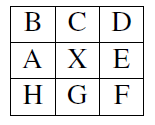
\includegraphics{superblok.png}
\caption{Blok X oraz jego 8-punktowe otoczenie}
\end{center}
\end{figure}

Przyk�adowo, dla bloku X z powy�szego rysunku mo�emy wyr�ni� nast�puj�ce superbloki:\{B,C,A,X\}, \{C,D,X,E\}, \{A,X,H,G\} oraz \{X,E,G,F\}.
W tej fazie algorytmu dla ka�dego superbloku kt�ry zawiera 3 bloki wype�nione t�em jest szacowany czwarty, brakuj�cy blok.Estymacja odbywa si� w dziedzinie cz�stotliwo�ci. Ka�da z omawianych metod skupia si� na analizie wysokich cz�stotliwo�ci, gdy� to one odpowiadaj� za zmienno�� obrazu. Faza ko�czy si� gdy ca�e t�o zostanie zrekonstruowane.
Omawiane dwa algorytmy r�ni� si� doborem transformaty.
\subsubsection{Estymacja z wykorzystaniem DCT}
 Metoda ta zosta�a zaproponowana w \cite{Reddy2009}. W tej metodzie dla ka�dego superbloku tworzone s� dwie r�ne wersje transformaty.
 \begin{enumerate}
 \item blok X jest zerowany, natomiast brana jest pod uwag� zawarto�� s�siednich blok�w. Na superbloku jest przeprowadzana dwuwymiarowa dyskretna transformata kosinusowa, a jej wsp�czynniki s� zapisywane w macierzy $C$ o wymiarach $M \cdot M$. Wsp�czynnik DC macierzy C (o wsp�rz�dnych (0,0)) jest ustawiany na 0, przez co pod uwag� zostanie wzi�te tylko przestrzenne zr�nicowanie warto�ci poszczeg�lnych pikseli. 
 \item bloki otaczaj�ce X s� zerowane, natomiast X jest inicjalizowany kolejnymi warto�ciami $r_k$ ze zbioru kandydat�w $R$ dla danej lokalizacji blokowej. Powstaje wi�c k wersji superbloku. Na ka�dym z superblok�w jest przeprowadzana 2D DCT, a jej wsp�czynniki s� zachowywane w macierzy $D_k$, gdzie k to numer kolejnego bloku ze zbioru kandydat�w. Tak jak poprzednio, wsp�czynnik DC macierzy $D_k$ jest ustawiany na zero. 
 \end{enumerate}
  
  Nale�y zauwa�y�, i� w wyniku zastosowania dw�ch przeciwstawnych masek superbloku (tj. zerowania okre�lonych blok�w do niego nale��cych) warto�ci pikseli w obszarze wysokich cz�stotliwo�ci b�d� przeciwstawne w macierzach $C$ oraz $D_k$. Maj� one r�wnie� tendencj� do redukowania si� przy dodawaniu tych macierzy. Istniej� jednak przypadki, gdy tak si� nie dzieje i w macierzach $C$ oraz $D_k$ nie ma element�w o wysokich cz�stotliwo�ciach - zdarza si� to gdy warto�ci pikseli w niewyzerowanych blokach sa bliskie zeru. Aby temu zapobiec, analizujemy �redni� pikseli $\mu_k$ bloku $r_k$ - je�li jest wy�sza lub r�wna 128, odpowiednie bloki w obu wersjach superbloku s� zerowane, a je�li �rednia jest ni�sza - wszystkie piksele tych blok�w s� ustawiane na 255. Korekta ta zapewnia, �e w ka�dym superbloku obszar wysokich cz�stotliwo�ci nie b�dzie pusty.
  
  W�asno�� redukowania si� wysokich cz�stotliwo�ci przy dodawaniu dw�ch komplementarnych superblok�w wykorzystano przy tworzeniu funkcji kosztu, wyznaczaj�cej najlepszy blok do uzupe�nienia brakuj�cego t�a. 
  Funkcja ta ma nast�puj�c� posta� 
  \begin{equation}
  \label{costfun}
  cost(k)=\left(\sum_{v=0}^{M-1}\sum_{u=0}^{M-1}\left|C(v,u)+D_k(v,u)\right|\right)\lambda_k
  \end{equation}
  \begin{equation}
  \lambda_k=e^{-\alpha\omega_k}
  \end{equation}
  
  gdzie $a\in\langle0,1\rangle$, $\omega_k=\frac{W_k}{\sum_{k=0}^{L-1}W_k}$, przy czym $W_k$ jest wag� elementu $r_k$, a L jest ilo�ci� element�w zbioru $r_k$. Wsp�czynnik $\alpha$ jest dobierany zazwyczaj eksperymentalnie i okre�la, jak du�y wp�yw na wynik funkcji kosztu ma waga danego bloku(czyli tak naprawd� cz�sto�� jego wyst�powania w sekwencji wideo). 
  Blok o najni�szej warto�ci funkcji kosztu (czyli taki, kt�ry najlepiej redukuje sum� wysokich cz�stotliwo�ci w macierzach C i D ) zostaje dodany jako najbardziej wiarygodna estymacja t�a.
   \subsubsection{Estymacja z wykorzystaniem rekursywnej transformaty Hadamarda}
   Metoda zosta�a przedstawiona po raz pierwszy w \cite{Baltieri2010} W tej metodzie ka�da ramka jest dzielona na bloki o rozmiarze $16 \cdot 16$ pikseli. Do przeprowadzenia trzeciego etapu tej metody jest wykorzystywana dyskretna transformata Hadamarda, b�d�ca generalizacj� transformaty Fouriera. Opiera si� ona na macierzach Hadamarda H, definiowanych rekursywnie w nast�puj�cy spos�b:
   \begin{equation}
    H_1=\left[1\right] \\
    \end{equation}
    \begin{equation}
   H_2N=\begin{bmatrix}
   H_N&H_N \\
   H_N&-H_N \\
   \end{bmatrix}
   \end{equation}
   
   Transformat� F bloku $X$ o wymiarach $2N \cdot 2N$ wyra�a si� jako
   \begin{equation}
   F=MXM
   \end{equation}
   gdzie M to macierz Hadamarda rz�du 2N. Bardzo u�yteczn� w�asno�ci� tej transformaty jest mo�liwo�� rozbicia jej na sum� transformat rz�du ni�szego. Przyk�adowo, po rozbiciu bloku X na podbloki A,B,C,D o wymiarach $N\cdot N$  transformat� mo�na obliczy� ze wzoru
   \begin{equation}F=
   \begin{bmatrix}
   H& H\\
   H & -H
   \end{bmatrix}
   \begin{bmatrix}
   A& B\\
   C& D
   \end{bmatrix}
      \begin{bmatrix}
      H& H\\
      H & -H
      \end{bmatrix}
   \end{equation}
gdzie H to macierz Hadamarda rz�du H.   
Wyra�aj�c macierz F jako:
\begin{equation}
\label{matrixf}
F=
\begin{bmatrix}
f_{1,1} & f_{1,2}\\
f_{2,1} & f_{2,2}
\end{bmatrix}
\end{equation}
otrzymujemy:
\begin{equation}
\label{matrixfelements}
\begin{cases} 
f_{1,1}=HAH+HBH+HCH+HDH\\ f_{1,2}=HAH-HBH+HCH-HDH\\
f_{2,1}=HAH+HBH-HCH-HDH\\ 
f_{2,2}=HAH-HBH-HCH+HDH\\ 
\end{cases}
\end{equation}
Stosuj�c wzory \ref{matrixf} oraz \ref{matrixfelements} mo�na obliczy� macierz Hadamarda rz�du 2N z czterech macierzy rz�du N, co b�dzie pomocne w przy wyliczaniu transformat superblok�w.
Tak samo jak w metodzie DCT, dla ka�dego superbloku tworzone s� 2 wersje transformat: pierwsza - z wyzerowanym blokiem X, bior�ca pod uwag� zawarto�� blok�w s�siednich oraz druga - z wyzerowanymi s�siednimi blokami, bior�ca pod uwag� tylko zawarto�� bloku X. Funkcja kosztu, okre�laj�ca kt�ry blok jest najlepszym kandydatem do bycia blokiem t�a, jest identyczna jak we wzorze \ref{costfun}. Algorytm wprowadza r�wnie� poprawk� na integralno�� wybranego bloku z reszt� t�a - je�li jego �redni gradient wzd�u� przynajmniej dw�ch kraw�dzi jest wi�kszy ni� $\gamma$, blok jest odrzucany, po czym nast�puje analiza kolejnego bloku z grupy kandydat�w z najmniejsz� warto�ci� funkcji kosztu.
Wsp�czynnik $\gamma$ jest dobierany eksperymentalnie.   
\chapter{Metodologia bada�}
\label{metodologia}
\section{U�yte sekwencje}
\label{sekwencje}
W niniejszej pracy do oceny jako�ci algorytm�w inicjalizacji t�a u�yto pierwszych 200 ramek nast�puj�cych sekwencji wideo:
\begin{enumerate}
\item clip\_01.mpg - sekwencja zarejestrowana przez kamer� umieszczon� na �cianie budynku C3 AGH w~pochmurny dzie�, przedstawiaj�ca ludzi chodz�cych po chodniku oraz cz�� jezdni ulicy Czarnowiejskiej wraz z~poruszaj�cymi si� na niej samochodami.
\item clip\_02.mpg - jak w~pkt. 1, lecz sekwencja jest zarejestrowana w~gorszej jako�ci obrazu.
\item clip\_03.mpg - jak w~pkt. 1, lecz przy zmiennych warunkach o�wietleniowych.
\item clip\_04.mpg - jak w~pkt. 1, lecz ze sta�ym cieniem.
\item fountain.mpg - sekwencja przedstawiaj�ca na pierwszym planie dzia�aj�c� fontann� na tle parkingu z~poruszaj�cymi si� samochodami.
\item highway.mpg - sekwencja zarejestrowana przez kamer� umieszczon� nad autostrad�.
\item pedestrians.mpg  - sekwencja zarejestrowana przez kamer� umieszczon� na dworcu kolejowym, przedstawiaj�ca poruszaj�cych si� po peronie pasa�er�w.
\item sidewalk.mpg - sekwencja zarejestrowana przez kamer� umieszczon� nad przej�ciem dla pieszych; na obrazie wyst�puj� mocne drgania kamery.
\end{enumerate}

\section{U�yte metryki}
W celu por�wnania skuteczno�ci algorytm�w dla ka�dej z~wy�ej wymienionych sekwencji zosta�y wyliczone modele t�a z~u�yciem r�nych metod i~wsp�czynnik�w. Obliczenia zosta�y przeprowadzone na ramkach w 8 bitowej skali szaro�ci.

Dla metod wykorzystuj�cych transformat� DCT oraz rekursywn� transformat� Hadamarda obliczenia zosta�y wykonane dla warto�ci wsp�czynnika $T_{corr} =  \{ 0.6, 0.7, 0.8, 0.9 \}$ oraz $T_{MAD} =  \{ 10, 20 \}$.

Tam, gdzie jest to mo�liwe zosta�a wybrana ramka referencyjna, najlepiej oddaj�ca t�o w~danej sekwencji. Nast�pnie obliczone modele t�a zosta�y przyr�wnane do tej�e ramki nast�puj�cymi metrykami:

\begin{enumerate}
\item B��d �redniokwadratowy (Mean Squared Error, MSE) 
\begin{equation}
MSE(I_r,I_b) = \frac{1}{N*M}\sum_{i=0}^{N-1}\sum_{j=0}^{M-1}(I_r(i,j)-I_b(i,j))^2
\end{equation}
Gdzie $I_r$ to ramka referencyjna, $I_b$ to obliczony model t�a, $N$ to wysoko��, a~$M$ to szeroko�� ramki

\item Procent podobie�stwa o~zadanym progu

Wsp�czynnik ten okre�la, ile pikseli w~wygenerowanym modelu t�a jest podobnych (z zadanym progiem) do odpowiadaj�cych pikseli w~ramce referencyjnej

\begin{equation}
P(I_r, I_b)= \sum_{i=0}^{N-1}\sum_{j=0}^{M-1} F(I_r(i,j), I_b(i,j))
\end{equation}

\begin{equation}
F(p_r, p_b)= 
\begin{cases} 
1, \, gdy \, |p_r-p_b|<(1-\alpha)*255\\
0, \, gdy \, |p_r-p_b|\ge(1-\alpha)*255\\
\end{cases}
\end{equation}
Gdzie $\alpha \in\space <0,1>$ oznacza wymagany pr�g podobie�stwa piksela, $I_r$ to ramka referencyjna, $I_b$ to obliczony model t�a,  $N$ to wysoko��, a~$M$ to szeroko�� ramki, $p_r$ to warto�� piksela ramki referencyjnej, $p_b$ to warto�� piksela wygenerowane modelu t�a.

\item Obraz r�nicowy

Metryka ta jest g��wnie przeznaczona do wizualnej oceny efektywno�ci algorytmu
\begin{equation}
AbsDiff(I_r, I_b)= |I_r - I_b|
\end{equation}

\end{enumerate}


\chapter{Badania}
\label{badania}

\section{Sekwencja clip\_01.mpg}
\begin{table}[ht]
\begin{tabular}{|*{18}{l|}}
\cline{1-17}
  \multirow{3}{*}{metryka} &
  \multicolumn{8}{|c|}{DCT} & \multicolumn{8}{|c|}{Hadamard} \\
\cline{2-18}
 & \multicolumn{4}{|c|}{10} & \multicolumn{4}{|c|}{20} & \multicolumn{4}{|c|}{10} & \multicolumn{4}{|c|}{20} & $T_{mad}$ \\
 \cline{2-18}
 & 0.6 & 0.7 & 0.8 & 0.9 & 0.6 & 0.7 & 0.8 & 0.9 &  0.6 & 0.7 & 0.8 & 0.9 & 0.6 & 0.7 & 0.8 & 0.9 & $T_{corr}$ \\
\hline
MSE\\ 
\cline{1-17}
PP (70 \% )\\
\cline{1-17}
PP (80 \% )\\
\cline{1-17}
PP (90 \% )\\
\cline{1-17}
PP (98 \% )\\
\cline{1-17}
\end{tabular}
\caption{Warto�ci metryk por�wnawczych dla metod pikselowych - sekwencja clip\_01.mpg}
\end{table}

\begin{table}[ht]
\begin{tabular}{|*{14}{l|}}
\cline{1-13}
 \multirow{2}{*}{metryka} &
 \multirow{2}{*}{�rednia}& \multirow{2}{*}{mediana} &
 \multirow{2}{*}{MOG} & \multicolumn{9}{|c|}{aproksymacja alfa} \\
 \cline{5-14}
 & & & & 0.1 & 0.2 & 0.3 & 0.4 & 0.5 & 0.6 & 0.7 & 0.8 & 0.9 & wsp�czynnik $\alpha$ \\
 \hline
 MSE \\ 
 \cline{1-13}
 PP (70 \%) \\ 
 \cline{1-13}
 PP (80 \%) \\ 
 \cline{1-13}
 PP (90 \%) \\ 
 \cline{1-13}
 PP (98 \%) \\ 
  \cline{1-13}
\end{tabular}
\caption{Warto�ci metryk por�wnawczych dla metod przestrzennych - sekwencja clip\_01.mpg}
\end{table}
\chapter{Por�wnania metod}

\chapter{S�ownik u�ytych poj��}
\label{slownik}

\begin{description}
\item[inicjalizacja t�a] proces jednorazowy, w kt�rym na podstawie pewnej ilo�ci ramek i odpowiednich algorytm�w zostaje uzyskany model t�a
\item[generecja t�a] ci�g�y proces aktualizacji wst�pnie zainicjalizowanego modelu  t�a
\item[blok] wydzielona kwadratowa cze�� ramki o~rozmiarach $N*N$, zawieraj�ca opr�cz pikseli informacj� o~wadze superbloku
\item[superblok] grupa 4~s�siaduj�cych ze sob� blok�w, tworz�ca wi�kszy blok(superblok) o~rozmiarach $2N * 2N$
\begin{figure}[ht]
\begin{center}
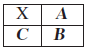
\includegraphics{blok.png}
\caption{Blok X~oraz jego otoczenie, tworz�ce razem z~nim superblok}
\end{center}
\end{figure}  
\item[grupa kandydat�w]
\item[lokalizacja blokowa]
\end{description}

% itd.
% \appendix
% \chapter{Dodatek A - spis zawarto�ci p�yty CD}

Do niniejszej pracy zosta�a do��czona p�yta CD zawieraj�ca foldery:
\begin{description}
\item[praca] - praca w formacie pdf
\item[praca\_latex] - praca w formacie \LaTeX
\item[sekwencje] - sekwencje u�yte do bada�
\item[kod] - kody �r�d�owe program�w napisanych w ramach pracy
\end{description}
% \chapter{Dodatek B - opis informatyczny programu}

W ramach niniejszej pracy zosta�y wykonane 2 programy napisane w j�zyku C++ przy u�yciu biblioteki OpenCV.
\section{Program robust}
Program \textbf{robust.exe} zawiera w sobie implementacj� 2 algorytm�w. S� nimi algorytm MOG oraz blokowy (przestrzenny), kt�ry w zale�no�ci od parametr�w wej�ciowych u�ywa transformaty Hadamarda lub DCT. 

Program ten przyjmuje parametry wej�ciowe w nast�puj�cej kolejno�ci:

\begin{enumerate}
\item �cie�ka do analizowanej sekwencji wideo,
\item wielko�� bufora ramek,
\item u�ywana metoda: 0 - MOG, 1 - metoda wykorzystuj�ca transformat� DCT, 2 - metoda wykorzystuj�ca transformat� Hadamarda,
\item rozmiar bloku (w przypadku wybrania metody MOG parametr ten pomija si�),
\item wsp�czynnik $T_{corr}$ (w przypadku wybrania metody MOG parametr ten pomija si�),
\item wsp�czynnik $T_{mad}$ (w przypadku wybrania metody MOG parametr ten pomija si�).
\end{enumerate}
Program sk�ada si� z nast�puj�cych klas
\subsection{blok}
Klasa blok przechowuje w kontenerze typu vector zawarto�� pojedynczego bloku. Posiada ona r�wnie� zmienn� weight, reprezentuj�c� wag� bloku oraz size, okre�laj�c� jego rozmiar. Jej najwa�niejsze metody to:
\begin{enumerate}
\item int getSize() - zwraca rozmiar bloku,
\item double mean() - oblicza �redni� z pikseli wchodz�cych w sk�ad bloku,
\item double deviation() - oblicza odchylenie standardowe z pikeli wchodz�cych w sk�ad bloku,
\item double corelation(blok \&blk) - oblicza wsp�czynnik korelacji z innym blokiem,
\item double mad(blok \&blk) - oblicza wsp�czynnik MAD z innym blokiem,
\item boolean similar(blok \&blk, double T1,double T2) - zwraca prawd�, je�li blok jest podobny do innego bloku przy wsp�czynniku korelacji r�wnym T1 i wsp�czynniku MAD r�wnym T2.
\end{enumerate}
\subsection{grid}
Klasa grid przechowuje ca�� siatk� grupy kandydat�w. Jej najwa�niejsze metody to:
\begin{enumerate}
\item void insertAt(int x,int y, blok\&) - wstawia do grupy kandydat�w dla lokalizacji blokowej o wsp�rz�dnych $(x,y)$ blok blk,
\item grid(int \_width, int \_height) - konstruktor, ustawiaj�cy wysoko�� i szeroko�� siatki,
\item void reserve(int n) - rezerwuje w pami�ci obszar do stworzenia siatki mog�cej pomie�ci� n element�w, musi by� wywo�ana po stworzeniu obiektu typu grid,
\item void fix() - naprawia b��dy zwi�zane z nieprawid�owo�ciami podczas przechwytywania obrazu (usuwa nieprawid�owe bloki z siatki) - musi by� wywo�ana po zako�czeniu kolekcjonowania kandydat�w.
\end{enumerate} 
\subsection{background}
Klasa background przechwouje odtworzone fragmenty t�a w kontenerze typu vector. Zawiera r�wnie� tablic� int**filltable, okre�laj�c�, czy dana lokalizacja blokowa posiada ju� odtworzone t�o (je�li tak, w tablicy w miejscu o wsp�rz�dnych x i y b�dzie znajdowa� si� warto�� 1) oraz licznik int nrfilled okre�laj�cy, ile fragment�w t�a zosta�o ju� odtworzonych. 
jej najwa�niejsze metody to:
\begin{enumerate}
\item Mat \& devectorize() - zwraca t�o jako obiekt Mat, kt�ry mo�na zapisa� i wy�wietli� przy u�yciu standardowych funkcji OpenCV,
\item void insertAt(int x,int y, blok\&) - wstawia dla lokalizacji blokowej o wsp�rz�dnych $(x,y)$ dany blok,
\item int isFilled(int x,int y) - zwraca ,,1'' gdy dla danej lokalizacji blokowej t�o zosta�o ju� odtworzone.
\end{enumerate}
\subsection{utils}
Utils jest klas� pomocnicz�, zawieraj�c� nast�puj�ce funkcje:
\begin{enumerate}
\item Mat** grid\_cut(Mat input\_image, int size) - zwraca ramk� obrazu w postaci tablicy obiekt�w Mat o danym rozmiarze - innymi s�owy dzieli j� na ma�e fragmenty,
\item - double cost(Mat C, Mat D,int size, double alpha, int weight) - liczy funkcj� kosztu dla transformaty, zgodnie ze wzorem (\ref{costfun}),
\item Mat hadamardmat(int size) - zwraca obiekt Mat b�d�cy macierz� Hadamarda o zadanym rozmiarze.
\end{enumerate}
\subsection{robust}
Robust jest to g��wna klasa, wykonuj�ca obliczenia na sekwencjach wideo i zwracaj�ca obrazy wynikowe t�a. Po uruchomieniu,gdy zostanie wywo�ana dla metod blokowych, tworzy ona pojedyncze obiekty klas grid(do przechowywania grupy kandydat�w) i background (do przechowywania odtworzonego t�a), a nast�pnie przetwarza ka�d� kolejn� ramk� zgodnie z algorytmem opisanym w sekcji \ref{blo:algorytm}. W przypadku wywo�ania jej dla metody MOG, u�ywa ona wbudowanej w OpenCV klasy BackgroundSubtractorMOG2, pozwalaj�cej obliczy� model t�a metod� MOG.
\section{Program simple\_pixel\_methods} 
Program \textbf{simple\_pixel\_methods.exe} zawiera w sobie implementacj� 3 algorytm�w. S� nimi algorytmy: �redniej z bufora, aproksymacji �redniej z bufora oraz mediany.

Program ten przyjmuje parametry wej�ciowe w nast�puj�cej kolejno�ci:

\begin{enumerate}
\item wielko�� bufora ramek,
\item typ metody (0 - aproksymacja, 1 - �rednia, 2 - mediana),
\item warto�� parametru $\alpha$ w przypadku wybrania metody aproksymacji.
\end{enumerate}

nie wiem co tu dalej napisa�...
% itd.

\bibliographystyle{alpha}
\bibliography{bibliografia}
%\begin{thebibliography}{1}
%
%\bibitem{Dil00}
%A.~Diller.
%\newblock {\em LaTeX wiersz po wierszu}.
%\newblock Wydawnictwo Helion, Gliwice, 2000.
%
%\bibitem{Lam92}
%L.~Lamport.
%\newblock {\em LaTeX system przygotowywania dokument�w}.
%\newblock Wydawnictwo Ariel, Krakow, 1992.
%
%\bibitem{Alvis2011}
%M.~Szpyrka.
%\newblock {\em {On Line Alvis Manual}}.
%\newblock AGH University of Science and Technology, 2011.cccccc
%\newblock \\\texttt{http://fm.ia.agh.edu.pl/alvis:manual}.
%
%\end{thebibliography}

\end{document}
